% This file is generated by the MATLAB m-file laprint.m. It can be included
% into LaTeX documents using the packages graphicx, color and psfrag.
% It is accompanied by a postscript file. A sample LaTeX file is:
%    \documentclass{article}\usepackage{graphicx,color,psfrag}
%    \begin{document}% This file is generated by the MATLAB m-file laprint.m. It can be included
% into LaTeX documents using the packages graphicx, color and psfrag.
% It is accompanied by a postscript file. A sample LaTeX file is:
%    \documentclass{article}\usepackage{graphicx,color,psfrag}
%    \begin{document}% This file is generated by the MATLAB m-file laprint.m. It can be included
% into LaTeX documents using the packages graphicx, color and psfrag.
% It is accompanied by a postscript file. A sample LaTeX file is:
%    \documentclass{article}\usepackage{graphicx,color,psfrag}
%    \begin{document}% This file is generated by the MATLAB m-file laprint.m. It can be included
% into LaTeX documents using the packages graphicx, color and psfrag.
% It is accompanied by a postscript file. A sample LaTeX file is:
%    \documentclass{article}\usepackage{graphicx,color,psfrag}
%    \begin{document}\input{Rs_SNR}\end{document}
% See http://www.mathworks.de/matlabcentral/fileexchange/loadFile.do?objectId=4638
% for recent versions of laprint.m.
%
% created by:           LaPrint version 3.16 (13.9.2004)
% created on:           01-Apr-2016 10:23:46
% eps bounding box:     16 cm x 12 cm
% comment:              
%
%\begin{psfrags}%
%\psfragscanon%
%
% text strings:
\psfrag{s05}[t][t]{\fontsize{8}{12}\fontseries{m}\mathversion{normal}\fontshape{n}\selectfont \color[rgb]{0,0,0}\setlength{\tabcolsep}{0pt}\begin{tabular}{c}$\snrrcvd = [\SI{}{dB}]$\end{tabular}}%
\psfrag{s06}[b][b]{\fontsize{8}{12}\fontseries{m}\mathversion{normal}\fontshape{n}\selectfont \color[rgb]{0,0,0}\setlength{\tabcolsep}{0pt}\begin{tabular}{c}$\e{ers}{\ers(\ttest)} = [\SI{}{bits/s/Hz}]$\end{tabular}}%
\psfrag{s10}[][]{\fontsize{10}{15}\fontseries{m}\mathversion{normal}\fontshape{n}\selectfont \color[rgb]{0,0,0}\setlength{\tabcolsep}{0pt}\begin{tabular}{c} \end{tabular}}%
\psfrag{s11}[][]{\fontsize{10}{15}\fontseries{m}\mathversion{normal}\fontshape{n}\selectfont \color[rgb]{0,0,0}\setlength{\tabcolsep}{0pt}\begin{tabular}{c} \end{tabular}}%
\psfrag{s12}[l][l]{\fontsize{8}{12}\fontseries{m}\mathversion{normal}\fontshape{n}\selectfont \color[rgb]{0,0,0}$\pcod = 0.99$}%
\psfrag{s13}[l][l]{\fontsize{8}{12}\fontseries{m}\mathversion{normal}\fontshape{n}\selectfont \color[rgb]{0,0,0}$\pcod = 0.90$}%
\psfrag{s14}[l][l]{\fontsize{8}{12}\fontseries{m}\mathversion{normal}\fontshape{n}\selectfont \color[rgb]{0,0,0}$\pcod = 0.95$}%
\psfrag{s15}[l][l]{\fontsize{8}{12}\fontseries{m}\mathversion{normal}\fontshape{n}\selectfont \color[rgb]{0,0,0}$\pcod = 0.99$}%
%
% axes font properties:
\fontsize{8}{12}\fontseries{m}\mathversion{normal}%
\fontshape{n}\selectfont%
%
% xticklabels:
\psfrag{x01}[t][t]{-10}%
\psfrag{x02}[t][t]{-5}%
\psfrag{x03}[t][t]{0}%
\psfrag{x04}[t][t]{5}%
\psfrag{x05}[t][t]{10}%
\psfrag{x06}[t][t]{15}%
%
% yticklabels:
\psfrag{v01}[r][r]{6}%
\psfrag{v02}[r][r]{6.5}%
\psfrag{v03}[r][r]{7}%
\psfrag{v04}[r][r]{7.5}%
\psfrag{v05}[r][r]{8}%
\psfrag{v06}[r][r]{8.5}%
\psfrag{v07}[r][r]{9}%
\psfrag{v08}[r][r]{9.5}%
\psfrag{v09}[r][r]{10}%
\psfrag{v10}[r][r]{10.5}%
\psfrag{v11}[r][r]{11}%
%
% Figure:
%\resizebox{8cm}{!}{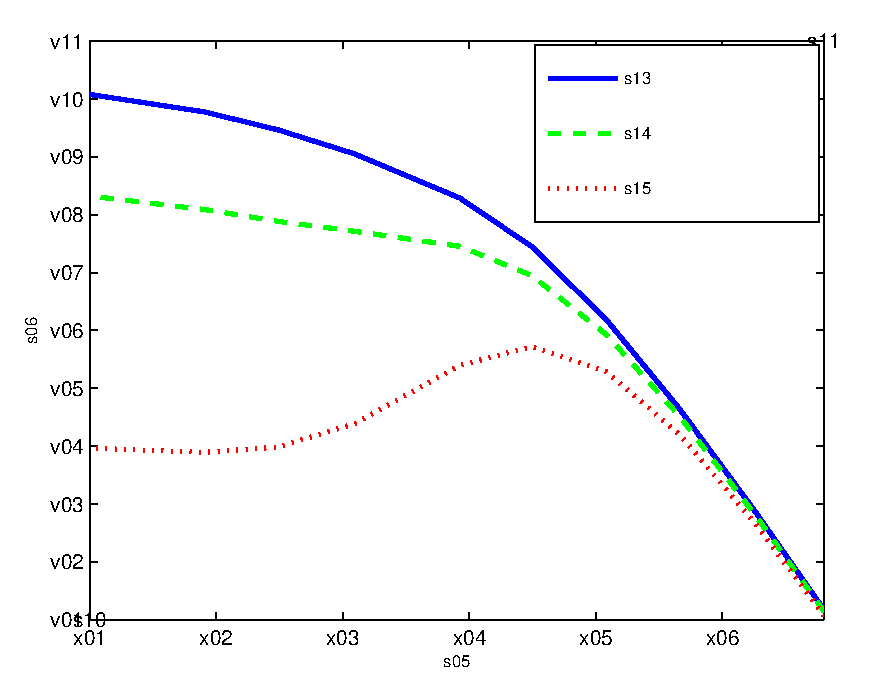
\includegraphics{Rs_SNR.eps}}%
%\end{psfrags}%
%
% End Rs_SNR.tex
\end{document}
% See http://www.mathworks.de/matlabcentral/fileexchange/loadFile.do?objectId=4638
% for recent versions of laprint.m.
%
% created by:           LaPrint version 3.16 (13.9.2004)
% created on:           01-Apr-2016 10:23:46
% eps bounding box:     16 cm x 12 cm
% comment:              
%
%\begin{psfrags}%
%\psfragscanon%
%
% text strings:
\psfrag{s05}[t][t]{\fontsize{8}{12}\fontseries{m}\mathversion{normal}\fontshape{n}\selectfont \color[rgb]{0,0,0}\setlength{\tabcolsep}{0pt}\begin{tabular}{c}$\snrrcvd = [\SI{}{dB}]$\end{tabular}}%
\psfrag{s06}[b][b]{\fontsize{8}{12}\fontseries{m}\mathversion{normal}\fontshape{n}\selectfont \color[rgb]{0,0,0}\setlength{\tabcolsep}{0pt}\begin{tabular}{c}$\e{ers}{\ers(\ttest)} = [\SI{}{bits/s/Hz}]$\end{tabular}}%
\psfrag{s10}[][]{\fontsize{10}{15}\fontseries{m}\mathversion{normal}\fontshape{n}\selectfont \color[rgb]{0,0,0}\setlength{\tabcolsep}{0pt}\begin{tabular}{c} \end{tabular}}%
\psfrag{s11}[][]{\fontsize{10}{15}\fontseries{m}\mathversion{normal}\fontshape{n}\selectfont \color[rgb]{0,0,0}\setlength{\tabcolsep}{0pt}\begin{tabular}{c} \end{tabular}}%
\psfrag{s12}[l][l]{\fontsize{8}{12}\fontseries{m}\mathversion{normal}\fontshape{n}\selectfont \color[rgb]{0,0,0}$\pcod = 0.99$}%
\psfrag{s13}[l][l]{\fontsize{8}{12}\fontseries{m}\mathversion{normal}\fontshape{n}\selectfont \color[rgb]{0,0,0}$\pcod = 0.90$}%
\psfrag{s14}[l][l]{\fontsize{8}{12}\fontseries{m}\mathversion{normal}\fontshape{n}\selectfont \color[rgb]{0,0,0}$\pcod = 0.95$}%
\psfrag{s15}[l][l]{\fontsize{8}{12}\fontseries{m}\mathversion{normal}\fontshape{n}\selectfont \color[rgb]{0,0,0}$\pcod = 0.99$}%
%
% axes font properties:
\fontsize{8}{12}\fontseries{m}\mathversion{normal}%
\fontshape{n}\selectfont%
%
% xticklabels:
\psfrag{x01}[t][t]{-10}%
\psfrag{x02}[t][t]{-5}%
\psfrag{x03}[t][t]{0}%
\psfrag{x04}[t][t]{5}%
\psfrag{x05}[t][t]{10}%
\psfrag{x06}[t][t]{15}%
%
% yticklabels:
\psfrag{v01}[r][r]{6}%
\psfrag{v02}[r][r]{6.5}%
\psfrag{v03}[r][r]{7}%
\psfrag{v04}[r][r]{7.5}%
\psfrag{v05}[r][r]{8}%
\psfrag{v06}[r][r]{8.5}%
\psfrag{v07}[r][r]{9}%
\psfrag{v08}[r][r]{9.5}%
\psfrag{v09}[r][r]{10}%
\psfrag{v10}[r][r]{10.5}%
\psfrag{v11}[r][r]{11}%
%
% Figure:
%\resizebox{8cm}{!}{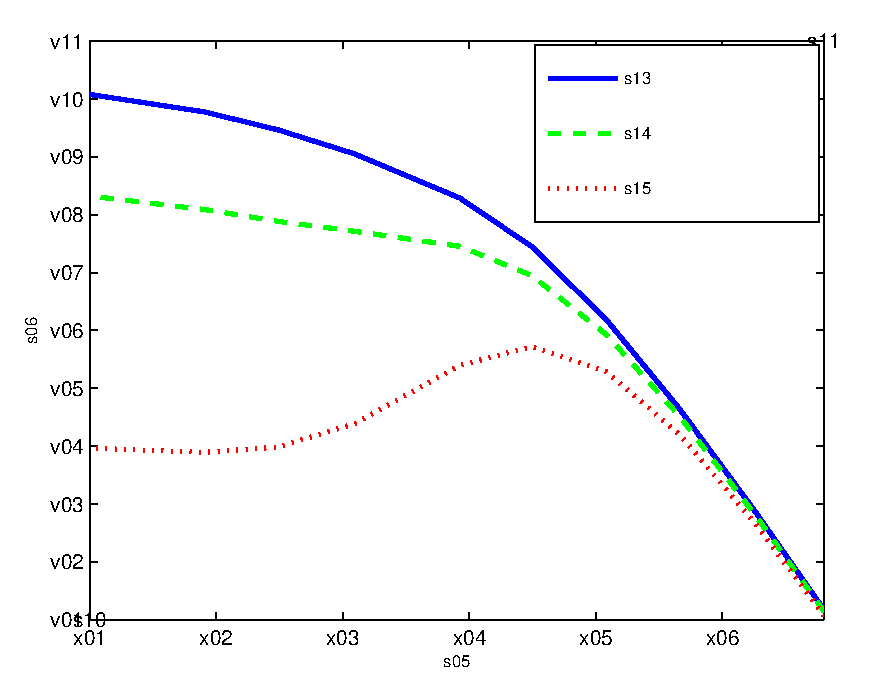
\includegraphics{Rs_SNR.eps}}%
%\end{psfrags}%
%
% End Rs_SNR.tex
\end{document}
% See http://www.mathworks.de/matlabcentral/fileexchange/loadFile.do?objectId=4638
% for recent versions of laprint.m.
%
% created by:           LaPrint version 3.16 (13.9.2004)
% created on:           01-Apr-2016 10:23:46
% eps bounding box:     16 cm x 12 cm
% comment:              
%
%\begin{psfrags}%
%\psfragscanon%
%
% text strings:
\psfrag{s05}[t][t]{\fontsize{8}{12}\fontseries{m}\mathversion{normal}\fontshape{n}\selectfont \color[rgb]{0,0,0}\setlength{\tabcolsep}{0pt}\begin{tabular}{c}$\snrrcvd = [\SI{}{dB}]$\end{tabular}}%
\psfrag{s06}[b][b]{\fontsize{8}{12}\fontseries{m}\mathversion{normal}\fontshape{n}\selectfont \color[rgb]{0,0,0}\setlength{\tabcolsep}{0pt}\begin{tabular}{c}$\e{ers}{\ers(\ttest)} = [\SI{}{bits/s/Hz}]$\end{tabular}}%
\psfrag{s10}[][]{\fontsize{10}{15}\fontseries{m}\mathversion{normal}\fontshape{n}\selectfont \color[rgb]{0,0,0}\setlength{\tabcolsep}{0pt}\begin{tabular}{c} \end{tabular}}%
\psfrag{s11}[][]{\fontsize{10}{15}\fontseries{m}\mathversion{normal}\fontshape{n}\selectfont \color[rgb]{0,0,0}\setlength{\tabcolsep}{0pt}\begin{tabular}{c} \end{tabular}}%
\psfrag{s12}[l][l]{\fontsize{8}{12}\fontseries{m}\mathversion{normal}\fontshape{n}\selectfont \color[rgb]{0,0,0}$\pcod = 0.99$}%
\psfrag{s13}[l][l]{\fontsize{8}{12}\fontseries{m}\mathversion{normal}\fontshape{n}\selectfont \color[rgb]{0,0,0}$\pcod = 0.90$}%
\psfrag{s14}[l][l]{\fontsize{8}{12}\fontseries{m}\mathversion{normal}\fontshape{n}\selectfont \color[rgb]{0,0,0}$\pcod = 0.95$}%
\psfrag{s15}[l][l]{\fontsize{8}{12}\fontseries{m}\mathversion{normal}\fontshape{n}\selectfont \color[rgb]{0,0,0}$\pcod = 0.99$}%
%
% axes font properties:
\fontsize{8}{12}\fontseries{m}\mathversion{normal}%
\fontshape{n}\selectfont%
%
% xticklabels:
\psfrag{x01}[t][t]{-10}%
\psfrag{x02}[t][t]{-5}%
\psfrag{x03}[t][t]{0}%
\psfrag{x04}[t][t]{5}%
\psfrag{x05}[t][t]{10}%
\psfrag{x06}[t][t]{15}%
%
% yticklabels:
\psfrag{v01}[r][r]{6}%
\psfrag{v02}[r][r]{6.5}%
\psfrag{v03}[r][r]{7}%
\psfrag{v04}[r][r]{7.5}%
\psfrag{v05}[r][r]{8}%
\psfrag{v06}[r][r]{8.5}%
\psfrag{v07}[r][r]{9}%
\psfrag{v08}[r][r]{9.5}%
\psfrag{v09}[r][r]{10}%
\psfrag{v10}[r][r]{10.5}%
\psfrag{v11}[r][r]{11}%
%
% Figure:
%\resizebox{8cm}{!}{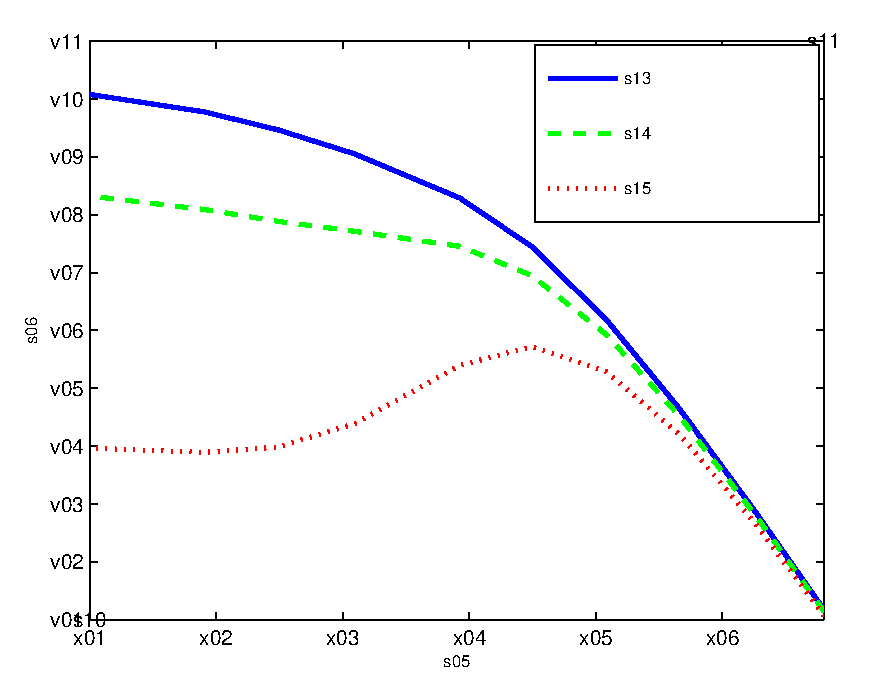
\includegraphics{Rs_SNR.eps}}%
%\end{psfrags}%
%
% End Rs_SNR.tex
\end{document}
% See http://www.mathworks.de/matlabcentral/fileexchange/loadFile.do?objectId=4638
% for recent versions of laprint.m.
%
% created by:           LaPrint version 3.16 (13.9.2004)
% created on:           23-Mar-2016 15:05:36
% eps bounding box:     16 cm x 12 cm
% comment:              
%
%\begin{psfrags}%
%\psfragscanon%
%
% text strings:
\psfrag{s05}[t][t]{\fontsize{8}{12}\fontseries{m}\mathversion{normal}\fontshape{n}\selectfont \color[rgb]{0,0,0}\setlength{\tabcolsep}{0pt}\begin{tabular}{c}$\snrrcvd = [\SI{}{dB}]$\end{tabular}}%
\psfrag{s06}[b][b]{\fontsize{8}{12}\fontseries{m}\mathversion{normal}\fontshape{n}\selectfont \color[rgb]{0,0,0}\setlength{\tabcolsep}{0pt}\begin{tabular}{c}$\e{ers}{\ers(\ttest)} = [\SI{}{bits/s/Hz}]$\end{tabular}}%
\psfrag{s10}[][]{\fontsize{10}{15}\fontseries{m}\mathversion{normal}\fontshape{n}\selectfont \color[rgb]{0,0,0}\setlength{\tabcolsep}{0pt}\begin{tabular}{c} \end{tabular}}%
\psfrag{s11}[][]{\fontsize{10}{15}\fontseries{m}\mathversion{normal}\fontshape{n}\selectfont \color[rgb]{0,0,0}\setlength{\tabcolsep}{0pt}\begin{tabular}{c} \end{tabular}}%
\psfrag{s12}[l][l]{\fontsize{8}{12}\fontseries{m}\mathversion{normal}\fontshape{n}\selectfont \color[rgb]{0,0,0}$\pcod = 0.99$}%
\psfrag{s13}[l][l]{\fontsize{8}{12}\fontseries{m}\mathversion{normal}\fontshape{n}\selectfont \color[rgb]{0,0,0}$\pcod = 0.90$}%
\psfrag{s14}[l][l]{\fontsize{8}{12}\fontseries{m}\mathversion{normal}\fontshape{n}\selectfont \color[rgb]{0,0,0}$\pcod = 0.95$}%
\psfrag{s15}[l][l]{\fontsize{8}{12}\fontseries{m}\mathversion{normal}\fontshape{n}\selectfont \color[rgb]{0,0,0}$\pcod = 0.99$}%
%
% axes font properties:
\fontsize{8}{12}\fontseries{m}\mathversion{normal}%
\fontshape{n}\selectfont%
%
% xticklabels:
\psfrag{x01}[t][t]{-10}%
\psfrag{x02}[t][t]{-5}%
\psfrag{x03}[t][t]{0}%
\psfrag{x04}[t][t]{5}%
\psfrag{x05}[t][t]{10}%
\psfrag{x06}[t][t]{15}%
%
% yticklabels:
\psfrag{v01}[r][r]{6}%
\psfrag{v02}[r][r]{6.5}%
\psfrag{v03}[r][r]{7}%
\psfrag{v04}[r][r]{7.5}%
\psfrag{v05}[r][r]{8}%
\psfrag{v06}[r][r]{8.5}%
\psfrag{v07}[r][r]{9}%
\psfrag{v08}[r][r]{9.5}%
\psfrag{v09}[r][r]{10}%
\psfrag{v10}[r][r]{10.5}%
\psfrag{v11}[r][r]{11}%
%
% Figure:
%\resizebox{8cm}{!}{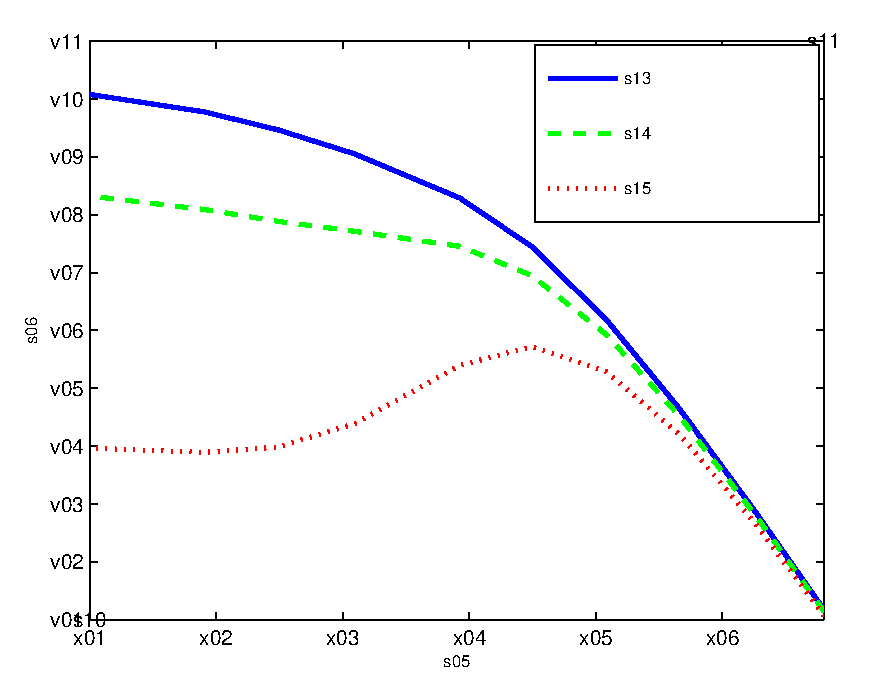
\includegraphics{Rs_SNR.eps}}%
%\end{psfrags}%
%
% End Rs_SNR.tex
